\chapter{Elementary Principles}
\section{Mechanics of a Particle}
\textbf{Linear Momentum}\\
Let $\textbf{r}$ be the radius vector of a particle from some given origin and $\textbf{v}$ its vector velocity.
$$\textbf{v}=\frac{d\textbf{r}}{dt}$$
The linear momentum $\textbf{p}$ of the particle is 
$$\textbf{p}=m\textbf{v}$$
Newton's second law of motion  states that there exist frames of reference in which the motion of the particle is described by the differential equation
$$\textbf{F}=\frac{d\textbf{p}}{dt}\equiv\dot{\textbf{p}}$$
$$\textbf{F}=\frac{d}{dt}(m\textbf{v})$$
If the mass of particle is constant
$$\textbf{F}=m\frac{d\textbf{v}}{dt}=m\textbf{a}$$
Where $\textbf{a}$ is the vector acceleration of the particle
The equation of motion is thus a differential equation of second order, assuming $\textbf{F}$ does not depend on higher-order derivatives.\\\\
\textbf{\textit{Conservation theorem for the Linear Momentum of a Particle: If the total force $\vec{F}$ is zero, then $\dot{\vec{p}}$, is conserved.}}\vspace{0.5cm}
\\\\
\textbf{Angular Momentum}\vspace{0.2cm}\\
The angular momentum of the particle about point $O$, denoted by $\textbf{L}$, is defined as
$$\textbf{L}=\textbf{r}\times\textbf{p}$$
where $\textbf{r}$ is the radius vector from $O$ to the particle. The moment of force or torque about $O$ 
 $$\textbf{N}=\textbf{r}\times\textbf{F}$$
 $$\textbf{r}\times\textbf{F}=\textbf{N}=\textbf{r}\times\frac{d}{dt}(mv)$$
 using the vector identity
 $$\frac{d}{dt}(\textbf{r}\times m\textbf{v})\textbf{v}\times m\textbf{v}+=\textbf{r}\times\frac{d}{dt}(m\textbf{v})$$
$$\textbf{N}=\frac{d}{dt}(\textbf{r}\times m\textbf{v})=\frac{d\textbf{L}}{dt}\equiv \dot{\textbf{L}}$$
Note that both $\textbf{N}$ and $\textbf{L}$ depend on the point $O$ about which the moments are taken.\\
\textit{Conservation Theorem for the Angular Momentum of a Particle: If the total torque, $\textbf{N}$,is zero then $\dot{\textbf{L}}=0$, and the angular momentum $\textbf{L}$ is conserved. }\\
\textbf{Energy}\\
Next consider the work done by the external force $\textbf{F}$ upon the particle in going from point 1 to point 2. \\
This work is 
$$W_{12}=\int\limits_{1}^{2}\textbf{F}\cdot d\textbf{s}$$
$$\int\textbf{F}\cdot d\textbf{s}=m\int\frac{d\textbf{v}}{dt}\cdot\textbf{v}dt=\frac{m}{2}\int\frac{d}{dt}(v^2)dt$$
$$W_{12}=\frac{m}{2}(v_2^2-v_1^2)$$
The scalar quantity $mv^2/2$ is called the kinetic energy of the particle and is denoted by $T$. so that the work done is equal to the change in the kinetic energy.
\begin{equation}
W_{12} =T_2-T_1\label{EP-01}
\end{equation}
if the force field is such that the work $W_{12}$ is the same for any physically possible path between points 1 and 2, then the force (and the system) is said to be conservative.\\
or
$$\oint\textbf{F}\cdot\textbf{s}=0 d$$
$\textbf{F}$ be the gradient of some scalar function of position
$$\textbf{F}=-\nabla V(\textbf{r})$$
where $V$ is called the potential energy.
$$\textbf{F}\cdot d\textbf{s}=-dV$$
or
$$F_s=-\frac{\partial V}{\partial s}$$
We can add to $V$ any quantity constant in space, without affecting  the results. Hence the zero level of $V$ is arnitrary.\\
For a consetvative system, the work done by the forces is 
\begin{equation}
W_{12}=V_1-V_2\label{EP-02}
\end{equation}
Combining Eq.(\ref{EP-01}) with Eq.(\ref{EP-02}),we have the result 
$$T_1+V_1=T_2+V_2$$
\textbf{\textit{Energy Consetvation Theorem for a Particle: If the forces acting on a particle are consetvative, then the total energy of the particle, $T+V$,is conserved}}\\
\begin{note}
	The force applied to to a particle may in some circumstances be given by the gradient of a scalar function that depends explicity on both the position of the particle and the time. However, the work done on the particle when it travels a distance $ds$.
	$$\textbf{F}\cdot{d\textbf{s}=\frac{\partial V}{\partial s}ds}$$
	is then no longer the total change in $-V$ during the displacement, since $V$ also changes explicitly with time as the particle moves. Hence, the work done as the particle goes from point 1 to point 2 is no longer the difference in the function $V$ between those points. While a total  energy $T+V$ may still be defined, it is not consetved during the course of the particle's motion.
\end{note}
\section{Mechanics of a system of Particle}
When considering a system of particles, we must distinguish between the external forces acting on the particles due to source outside the system and internal forces on some particle $i$ due to all other particles in the system.\\\\
\textbf{Linear Momentum}\\
Equation of motion for the $i^{th}$ particle
$$\vec{F}_i^{(e)}+\sum\limits_{j}\vec{F}_{ji}=\vec{\dot{p}_i}$$
$\vec{F}_i^{(e)}$- external force\\
$\vec{F}_{ji}$- internal force on the $i^{th}$ particle due to the $j^{th}$ particle.\\\\
Assume $\vec{F}_{ij}$ , like ${F}_i^{(e)}$ obey Newton's third law  ie. $\vec{F}_{ij}= - \vec{F}_{ji}$,\\
this assumption some times referred to as \textit{The weak law of action and reaction}.\\
$$\therefore \text{ we get }\quad \frac{d^2}{dt^2}\sum\limits_{i}m_ir_i=\sum\limits_{i}{F}_i^{(e)}+\sum\limits_{i,j ,\ i\neq j}F_{ji}$$
$$\frac{d^2}{dt^2}\sum\limits_{i}m_ir_i=\sum\limits_{i}{F}_i^{(e)}$$
Let's define $\vec{R}$ as the average of radii vectors of the particles weighted in proportion to their mass.
$$\vec{R}=\frac{\sum m_i \vec{r}_i}{\sum m_i}=\frac{\sum m_i \vec{r}_i}{M}$$
vector $\vec{R}$ defines a point known as the centre of mass
$$M\frac{d^2 R}{dt^2}=\sum\limits_{i}\vec{F}_i^{(e)}\equiv \vec{F}^{(e)}$$
The centre of mass moves as if the total external force were acting on the entire mass of the system concentrated at the centre of mass. The total limear momentum of system.
$$\vec{P}=\sum m_1\frac{d\vec{r_i}}{dt}=M\frac{d\vec{R}}{dt}$$
ie. total mass of the system times the velocity of the center of mass\\
conservation for linear momentum of a system of particles: if the total external force is zero, the total linear momentum is conserved.\\\\
\textbf{Angular Momentum}\\
\begin{align*}
\sum\limits_{i}(\vec{r_i}\times\dot{P_1})&=\sum\limits_{i}\frac{d}{dt}(\vec{r_i}\times\vec{P_i})=\dot{L}\\
&=\sum\limits_{i}\vec{r_i}\times\vec{F}_i^{(e)}+\sum\limits_{i,j}\vec{r_i}\times\vec{F}_{ji}\\
\vec{r_i}-\vec{r_j}&=\vec{r_{ij}}\\
\therefore \text{ RHS of equation becomes },\quad\vec{r_{ij}}\times \vec{F_{ji}}
\end{align*}
The internal forces between two particles. in addition to being equal and opposite, also lie along the line going the particles (This condition known as the strong law of action and reaction.)\\
Then all cross products vanish,\\
$$\frac{d\vec{L}}{dt}=\vec{N}^{(e)}$$\\
The time derivative of angular momentum thus equal to the moment of the external force about the given point.\\\\
Conservation of total angular momentum: $L$ \textit{is constant in time if the applied (external) torque is zero.} \\\\\begin{note}
	This is a vector theorem,
	$\therefore$ $L_z$ will be conserved if $N_z^{(e)}$ is zero, even if $N_x^{(e)}$ and $N_y^{(e)}$ are not zero.\\
\end{note} 
\textbf{To represent $\vec{L}$ in terms of centre of mass,}\\
\begin{figure}[H]
	\centering
	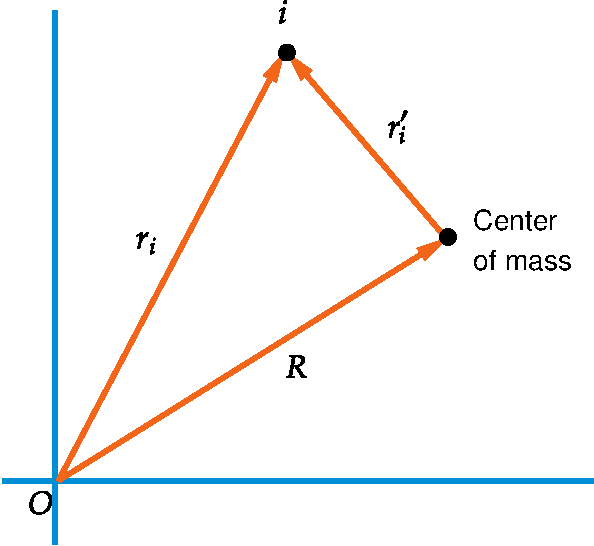
\includegraphics[height=4cm,width=5cm]{EP-02}
\end{figure}
Let $R$ be the radius vector from $O$ to the centre of mass to the $i^{th}$ particle\\
\begin{align*}
\vec{r_1}&=\vec{r^\prime_1}+\vec{R}
\intertext{and}
\vec{v_1}&=\vec{v^\prime_1}+\vec{\mathrm{v}}
\intertext{where}
\mathrm{v}=\frac{dR}{dt}\text{velocity of CM relative to $O$ }
\intertext{and}
v^\prime_1=\frac{dr^\prime}{dt}
\end{align*}
is the velocity of the $i^{th}$ particle relative to centre of mass of the system\\
$\therefore$ total angular momentum
$$\vec{L}=\vec{R}\times M\vec{\mathrm{v}}+\sum\limits_{i}r^\prime_i\times p^\prime_i$$
Total angular momentum about a point $O$ is the angular momentum of motion concentrated at the centre of mass, plus the angular momentum of motion about the centre of mass.\\
\begin{note}
	$L$ depends on origin $O$ through the vector $\vec{R}$ 
	only if the centre of mass is at rest with respect to $O$ will the angular momentum be independent of point of reference.
\end{note}

